\def\year{2019}\relax
%File: formatting-instruction.tex
\documentclass[letterpaper]{article} %DO NOT CHANGE THIS
\usepackage{aaai19}  %Required
\usepackage{times}  %Required
\usepackage{helvet}  %Required
\usepackage{courier}  %Required
\usepackage{url}  %Required
\usepackage{graphicx}  %Required
\usepackage{booktabs}
\usepackage{multirow}
\usepackage{algorithm}
\usepackage{algorithmic}
\usepackage{listings}
\usepackage{amsfonts}
% \usepackage{float}
\usepackage{subfigure}
% \usepackage{latexsym}
\usepackage{amsmath}
\frenchspacing  %Required
\setlength{\pdfpagewidth}{8.5in}  %Required
\setlength{\pdfpageheight}{11in}  %Required
%PDF Info Is Required:
  \pdfinfo{
/Title (2019 Formatting Instructions for Authors Using LaTeX)
/Author (AAAI Press Staff)}
\setcounter{secnumdepth}{0}  
 \begin{document}
% The file aaai.sty is the style file for AAAI Press 
% proceedings, working notes, and technical reports.
%
\title{Knowledge Association Network for Measuring Semantic Relatedness}
\author{
}
\maketitle              % typeset the header of the contribution
  %
  \begin{abstract}
    Measuring semantic relatedness between two words is a fundamental task for many applications in Natural Language
    Processing(NLP). Conventional methods mainly utilize the latent semantic hidden in lexical database(WordNet) or text corpus(Wikipedia).
    They make great achievements based on the distance computing in lexical tree or co-occurrence principle in Wikipedia.
    However these methods suffer from low coverage and low precision because
    1) lexical database contains abundant lexical information but lacks the semantic information;
    2) in Wikipedia, two related words may not appear in a window size e.g. synonyms, and two unrelated words may 
    be mentioned together by chance. To compute semantic relatedness more accurately, some other approaches make great efforts
    based on free association network and get an significant improvement on relatedness measurement. Nevertheless,
    they need complex preprocessing in Wikipedia. Besides, the fixed score functions they adopt cause the lack of
    flexibility and expressiveness of model. 
    In this paper, we explore knowledge graph(DBPedia) and wikipedia to construct a knowledge association network which avoids the
    preprocessing of Wikipedia. And we use distributed vectors instead of fixed score functions to represent the attributes
    and topological structure of our network respectively. The experiment based on gold dataset shows that our model outperforms
    the state-of-the-art models.

    % Measuring semantic relatedness between two words is a fundamental task for many applications in Natural Language Processing(NLP). Conventional methods mainly utilize the latent semantic hidden in lexical database(WordNet) or text corpus(Wikipedia). The methods based on lexical database measure the relatedness between two words using fixed semantic, such as the distance between them or the nearest parent node they share. The Wikipedia-based methods regard two words highly related if they appear in a special window size(co-occurrence principle). Such methods suffer from low coverage and low precision because 1) lexical database contains abundant lexical information but lacks the semantic information; 2) In co-occurrence principle of Wikipedia, two related words may not appear in a window size e.g. synonyms, and two unrelated words may be mentioned together by chance. To compute semantic relatedness more accurately, we explore the latent semantics in knowledge graph(DBPedia) and construct a knowledge association network. We use distributed vectors to represent the attributes and topological structure of such network respectively. The experiment based on gold dataset shows that our model outperforms the state-of-the-art models.

  \end{abstract}

  \section{Introduction}
% problem description: semantic relatedness
Computing semantic relatedness(SR) between two elements(words, sentences,
texts etc.) is a fundamental task for many applications in Natural Language
Processing(NLP) such as lexicon induction\cite{aaai/QadirMGL15}, Named 
Entity Disambiguation\cite{acl/HanZ10}, Keyword Extraction
\cite{ijcai/ZhangFW13} and Information Retrieval\cite{acl/GurevychMZ07}. 
Additionaly, computing semantic relatedness contributes other applications, 
for example, opinion spam problem\cite{www/SandulescuE15}, image classification\cite{iwcs/LeongM11} and so on. 
In this paper we focus on computing semantic relatedness between two 
words in knowledge graph.

It has long been thought that when humans measure the relatedness between
a pair of words, a deeper reasoning is triggered to compare the concepts
behind the words. Many traditional studies on semantic relatedness
utilize different data sources. There are
i) \emph{the large corpora}, such as wikipedia\cite{ijcai/GabrilovichM07},
ii) \emph{the lexical databases}, such as WordNet\cite{acl/Pucher07} or Wikithionary\cite{aaai/ZeschMG08}, 
iii) \emph{the knowledge graph}, such as DBpedia\cite{aaai/NavigliP12} or BabelNet\cite{aaai/NavigliP12}.
With the development of knowledge representation, utilizing knowledge-rich resources to compute semantic 
relatedness is a well-explored line of research. It is known to all that
knowledge graph contains richer syntactic and semantic information than lexical databases,
and more structured knowledge than the large corpora.
On the account of advantages of knowledge graph, we utilize it as background 
knowledge to compute semantic relatedness.

% Knowledge graph can be accessed with powerful query language Sparql in RDF graph.
% As for the methods build on the data soruce, the recent word embedding 
% learning approaches demonstrate their abilities
% to capture syntactic and semantic information, and outperform the
% lexicon-based methods\cite{acl/Pucher07}. 
% Knowledge Graph, as a semantic graph, stores
% vast amount of structured knowledge. 

Recently, there are some researchers having attached importance to measure semantic relatedness
in knowledge graph\cite{acl/IacobacciPN15}, \cite{aaai/NavigliP12}, \cite{aaai/Pirro12}. 
This paper \cite{acl/IacobacciPN15} leveraged entity linking to annotate the dump of wikipedia. Based on this,
the sense-annotated corpus was generated. Then they\cite{acl/IacobacciPN15} used word2vec to
train the sense-annotated corpus and got distributed representation of different 
word senses. This step still needs a significant preprocessing and data transformation efforts. 
As we can see that the author\cite{acl/IacobacciPN15} computed semantic relatedness on account of large corpora.
They just put the knowledge graph on the position of support.
Another paper\cite{aaai/NavigliP12} proposed a knowledge-rich approach to compute multilingual semantic
relatedness which exploited the joint contribution of different languages. Given a pair of words 
in two languages, they\cite{aaai/NavigliP12} utilized BabelNet to collect their translations and computed semantic
relatedness in a variety of languages. Then they combined the empirical evidence from these 
different languages by intersecting their respective graphs.
Another work \cite{aaai/Pirro12} proposed an approach which exploited the graph nature of RDF and SPARQL query
Language to access knowledge graph. It not only obtained the comparable
result with the state-of-art model at that moment, but also avoided the burden
of preprocessing and data transformation.

Though the paper\cite{aaai/Pirro12} avoided a significant preprocessing and data
transformation effort, and develops scalability of their approach while adopting 
the knowledge graph. However, they missed some factors which
might contribute to semantic relatedness measurement. Firstly, given two words
as input, the first step is to find corresponding entities in knowledge
graph. Obviously, there are usually more than one corresponding entities for a single word.
For an input word \emph{car}, for example, we will get \emph{DBPedia:\footnote{http://dbpedia.org/resource}Automobile} and
\emph{DBPedia:Auto\underline{\hspace{0.5em}}Racing} and so on. The work \cite{aaai/Pirro12} losed
sight of the informativeness of the other entities, while they just
consider the entity with the highest rank. Secondly, they \cite{aaai/Pirro12} misseed
some informativeness of \emph{objects} in \emph{triple(subject, prediacte, object)} because their strategy took
the \emph{predicates} into account exclusively based on the TFIDF. This
method ignored the function of \emph{objects} in a semantic triple.

\begin{figure*}
    \centering
    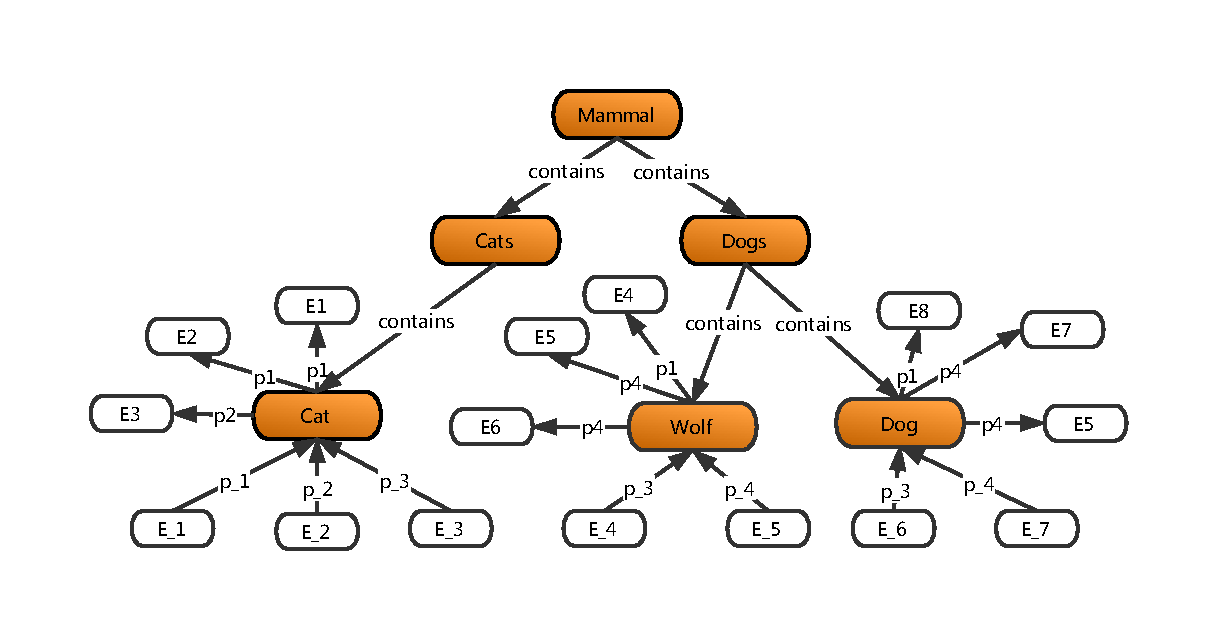
\includegraphics[width=1.1\textwidth]{pic/introduction.pdf}\\
    \caption{Subgraph example in knowledge graph}
    \label{weak1}
\end{figure*}

As show in figure \ref{weak1}, the subgraph contains \emph{Dogs} and \emph{Cats} extracted from
knowledge. We simplify the specific features of \emph{Dogs} and \emph{Cats} to concise symbol shown as $E_i$ in figure. 
We can see that the entity \emph{Cat} plays the role 
of both \emph{Object(Cats contains Cat)} and \emph{Subject(Cat $p_1$ $E_1$)}
in the pattern of triples. The \emph{predicate} which is connected with an entity(Cat)
may be regarded as an outgoing($p_1$) or incoming \emph{predicate}($p_{_1}$).
In the paper\cite{aaai/Pirro12}, the relatedness space for an entity ${E_i}$ is modelled as a 
$k$-dimensional weighted vector \emph{V$_i$}, where each dimension represents
the informativeness of a specific \emph{predicate}.
For example, the weighted vector for \emph{Cat} is 
$[v_{p_1}^o, v_{p_2}^o, v_{p_\_1}^i, v_{p_\_2}^i, v_{p_\_2}^i]$ in which $v_{p_i}^o$ 
means the vector value of outgoing predicate $p_i$ and $v_{p_j}^i$ 
means the vector value of incoming predicate $p_j$.
In this example, from the view of outgoing \emph{predicate} $p_i$, there are three triples
\emph{(Cat $p_1$ $E_1$)}, \emph{(Cat $p_1$ $E_2$)} and \emph{(Cat $p_2$ $E_3$)} which describe the entity \emph{Cat}.
Specifically, in order to compute the vector value of $p_1$,
the way of paper \cite{aaai/Pirro12} in which they got the informativeness of $p_i$ was to count the number
of triples with the form of \emph{(Cat $p_1$ ?)} firstly, then they divided this result
by the total number of triples in which \emph{Cat} appears
((Cat $p_1$ $E_1$), (Cat $p_1$ $E_2$), (Cat $p_2$ $E_3$)), i.e., $v_{p_1}^o$=2/3.
They\cite{aaai/Pirro12} only considered the informativeness of \emph{prediacte},
and ignored the function of a set of specific \emph{objects} in a pattern of triple.
Besides, there is another aspect they have ignored. In this example, for entities $Cat$,
$Dog$ and $Wolf$, let us see the informativeness of prediacte $p_1$. We get
\emph{(Cat $p_1$ $E_1$), (Cat $p_1$ $E_2$), (Wolf $p_1$ $E_4$)} and \emph{(Dog $p_1$ $E_8$)}. 
It is obvious that when they\cite{aaai/Pirro12} computed relatedness between \emph{Cat} and \emph{Wolf}, 
they got the same vector value for predicate $p_1$ both in the aspect of \emph{Wolf} and \emph{Dog}.
In other words, in the dimension of predicate $p_1$ vector between pair (\emph{Cat},\emph{Wolf}) and
(\emph{Cat},\emph{Dog}), they got no difference. Accordingly, they did not distinguish the different
objects for a specific predicate. In order to improve the performance of 
semantic relatedness measurement based on knowledge graph, we propose a threefold model which is shown as follows:

1. For given a pair of words, the first job is to query the corresponding entities. In order to use the
neural network for training the dataset, we also need to construct a graph which contains all related
entities, attributes and relations between the corresponding entity pairs.

2. We use Starspace proposed by Facebook for knowledge graph instead of Word2vec to train the subgraph
extracted from the knowledge graph. Then we can get a distributional representation(vector) for each
entity and predicate. 

3. When we take as inputs a pair of words, we can get two sets of corresponding entities queried from
knowledge graph. Then we can get multiple relatedness scores after a full link between these two sets of entities.
Inspired by \cite{acl/IacobacciPN15}, we utilize an approach to combine the 
relatedness scores as the final semantic relatedness score in knowledge graph.

This paper is organized as follows. We give the related work about semantic relatedness
measurement in section \ref{related-word}. Then we elaborate the threefold model for
computing relatedness scores in section \ref{methodlogy}. Finally, we display detailed
illustrations of experiment results which show that our model outperform the state-of-the-art model.
  \section{Knowledge Association Network}
\label{kan}
It has long been thought that when humans measure the relatedness between a pair of words,
a deeper reasoning which requires a large amount of knowledge is triggered to compare the concepts behind the words.
There are many data resources that contain concepts which are associate with words such as Wikipedia, Wordnet and DBPedia etc.
Wordnet provides precise lexical information but lacks adequate semantic information.
Wikipedia is a large corpus where a page describes a concept.
DBPedia contains abundant structured knowledge consisting of a great number of facts which are extracted from wikipedia. 

Inspired by the free association network in semantic relatedness between two words\cite{aaai/GongXH18,aaai/ZhangZH15}, 
we consider the DBPedia as concepts database to avoid the significant preprocessing and data transformation efforts in wikipedia. 
To measure the relatedness between two entities, we consider two major factors in DBPedia: attributes information and topological structure. 
The attributes of an entity include the properties, categories, ontology information and some other information which enhances
the entity itself. Topological structure reflects the relations between other
entities on the basis of a special predicate in DBPedia: \emph{WikiPageRedirectOf}.
That means if two entities are connected by this predicate, they appear in the same Wikipedia page.

\begin{figure}
    \flushleft
    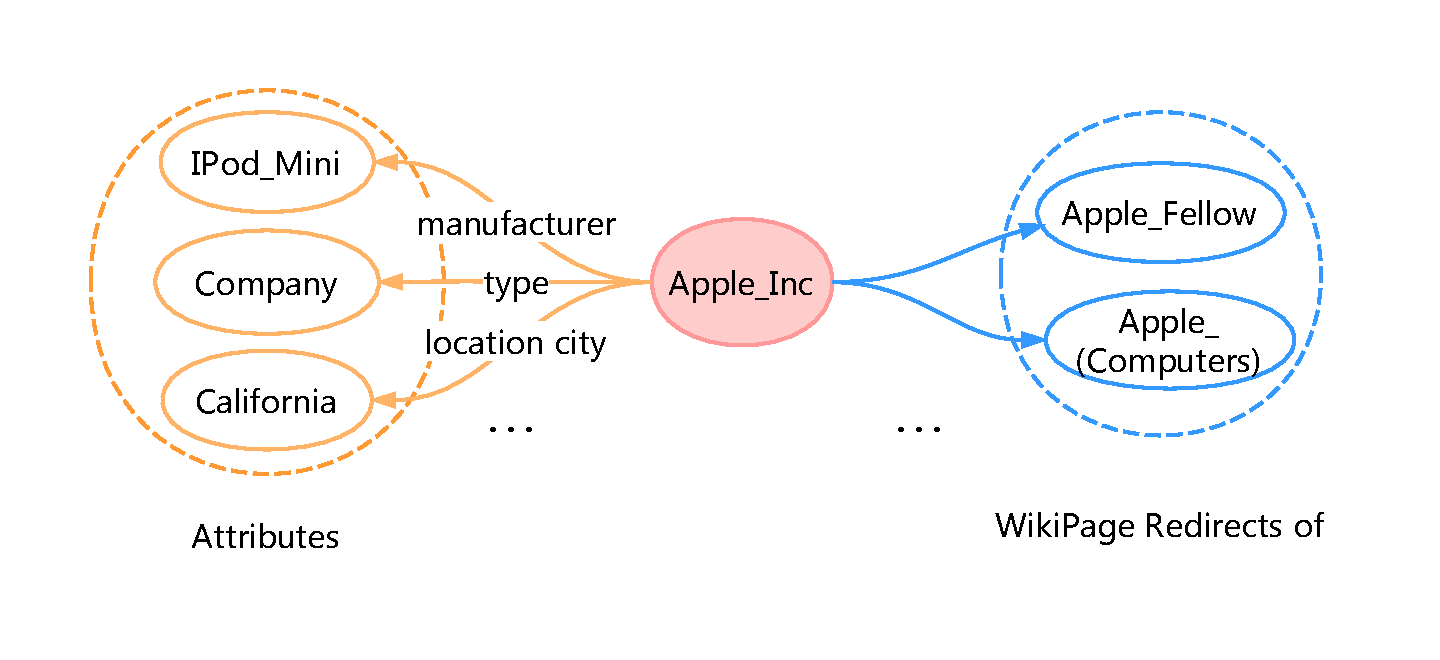
\includegraphics[width=0.5\textwidth]{pic/kg.pdf}\\
    \caption{The semantics around an entity}
    \label{kg}
\end{figure}

There is an example in figure \ref{kg}, for the technology company Apple which is described
as \emph{Apple Inc} in DBPedia, we get its attributes, that is, "Apple is the manufacturer of IPod Mini(properties)"; "Apple is a company(categories)" and etc.
And the relationship descriptions(\emph{predicates in triples)} are named on the basis of ontology language that contains affluent semantics.
In the aspect of links among other co-occurrence entities, there are entities \emph{Apple\_Fellow} and \emph{Apple\_(Company)} in accordance with the
special relationship \emph{WikipageRedirectOf}.

DBPedia contains natural attributes network structure and abundant semantics.
We define a set of entities $\mathit{E_w=\{e_1, e_2, ..., e_i\}}$ that represent the semantics behind a word and $e_i$ is an entity in DBPedia.
We refer to the attributes of an entity as an attributes graph $\mathit{G_{attr}=\{a_1, a_2, ..., a_j\}}$ and define topological structure as 
$\mathit{G_{t}=G(E, R_{redirect})}$, where $a_i$ denotes an attribute and $E$ is a set of entities, $R_{redirect}$ is the edge set formed by
\emph{WikiPageRedirectOf}.

\subsubsection{Definition}
\emph{Knowledge association network can be modelled as a graph $G=(W, E, R)$ where $w$ is the word set in vocabulary, $E$ is the entity set contained in DBPedia,
and edge set $R$ denotes the relationships including word-to-word($R_{w}$), entity-to-entity($R_{e}$), and word-to-entity($R_{we}$).}

\subsubsection{Network Construction}
A necessary work in network construction is to build the mapping between words and concepts(entities). 
This comes in handy in Wikipedia pages. The mapping between words and Wikipedia page reflects 
the structure of association network naturally, and fortunately there is a 1-to-1 match between entity in DBPedia and page in Wikipedia.
In other words, Wikipedia page and it's corresponding DBPedia entity elaborate the same concept.
Consequently we can construct knowledge association network based on this natural mapping.

There is a special attribute called \emph{WikipageID} that reflects the mapping between entities in DBPedia and pages
in Wikipedia by the unique id.
The id can be obtained by the \emph{Gensim}\footnote{https://radimrehurek.com/gensim/wiki.html} that is a free Python
library designed to automatically extract semantic topics from documents. By the aid of unique page id,
we get the unique corresponding entity in DBPedia by SPARQL endpoint\footnote{http://dbpedia.org/sparql}.
For example, the id of Wikipedia page \emph{Apple Inc} is $856$, we can use a simple query to get the unique entity name \emph{Apple\_Inc}:

\begin{lstlisting}[basicstyle=\fontsize{9}{11}\ttfamily]
PREFIX dbo: <http://dbpedia.org/ontology/>
SELECT ?E WHERE {
    ?E dbo:wikiPageID 856.
}
\end{lstlisting}


  \section{Semantic Relatedness Measurement}
\label{sr}
We give an overview of our model in figure \ref{overview} where solid lines lead the flow of model and dotted lines
demonstrate that there is an additional function from source part to target part. \
This figure illustrates the construction of our network and the relatedness measurement.
For the words in vocabulary, we can get a mapping between words and concepts(pages in Wikipedia)
by corpus statistics. Then we query the unique entity by the page id in DBPedia SPARQL endpoint.
For the layer of entity-to-entity, we divide it into attributes and topological structure and embed them by different models. 
As for the semantic relatedness computing, we consider three layers relatedness measurement:
word-to-word, word-to-entity and entity-to-entity when it comes to knowledge association network.

\begin{figure*}
    \flushleft
    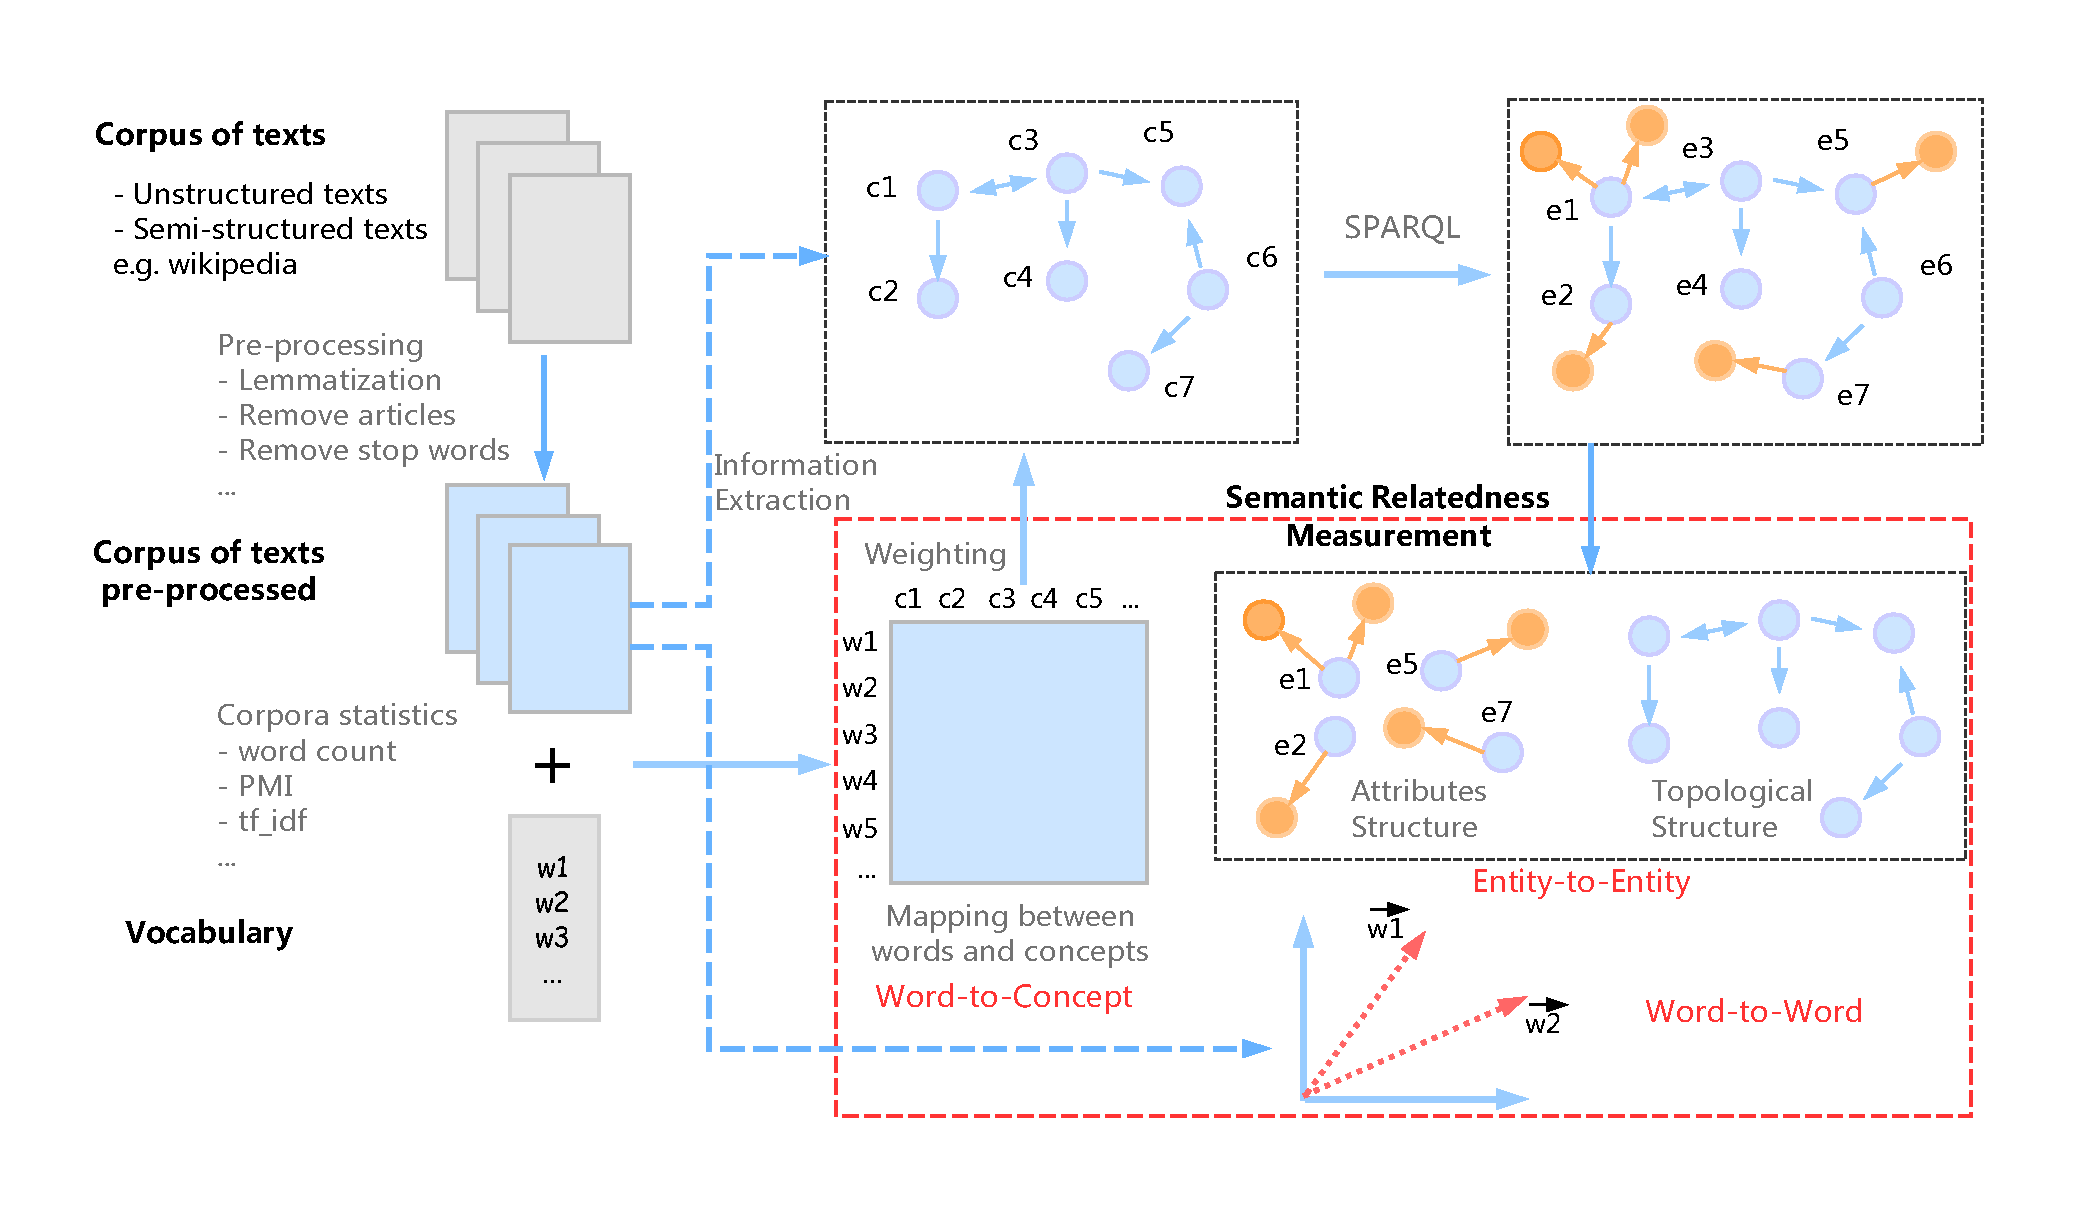
\includegraphics[width=1\textwidth]{pic/association-network.pdf}\\
    \caption{Association Network in Semantic measurement}
    \label{overview}
\end{figure*}

\subsection{word-to-word}
The semantic relatedness in word layer is mainly measured by 1) distributed vector representation such as word2vec \cite{corr/Mikolov13} 
and GloVe \cite{emnlp/PenningtonSM14} etc. 2) word co-occurrence, which means two words are relevant if they appear in a window size K. 
Experimental results prove that distributed vector representation works better in computing semantic relatedness\cite{corr/Mikolov13}.
Therefore in this paper, we abandon co-occurrence-based methods and adopt word2vec to train the Wikipedia corpus to product effective
vector representation for each word. 
Let $\overrightarrow v_i$ and $\overrightarrow v_j$ denote the vector representation of $w_i$ and $w_i$, and $f(w_i, w_j)$ is the semantic
relatedness score. The vector representation can be utilized to calculate the semantic relatedness based on cosine
function. Formally, we get:

\begin{small}
    \begin{equation}
        \label{cos}
        % \nonumber
        f_w(w_i, w_j) = cos(\overrightarrow v_i,\overrightarrow v_j) = \frac{\overrightarrow v_i \cdot 
        \overrightarrow v_j}{\left \| \overrightarrow v_i \right \|\left \| \overrightarrow v_j \right \|}
    \end{equation}
\end{small}

The word2vec algorithms include skip-gram and CBOW models, using either hierarchical softmax or negative sampling.
The combination of skip-gram and negative sampling are used frequently and effective experimentally. We choose this
training program accordingly. The detailed parameter setting can be seen in the part of experiment.

\subsection{word-to-entity}
In the knowledge association network, there is a one-to-many relationship between words and entities in DBPedia.
For a given word, several relevant entities will rise from our network due to the word ambiguity.
To measure the degree of association between word($w$) and entity($e$), 1) some researchers\cite{aaai/Pirro12}
take the co-occurrence times between $w$ and $c$ as the judgement of relatedness,
which is insensitive for some common words like \emph{this}, \emph{that} and so on. 
2) and some other related works\cite{aaai/GongXH18} consider $w$ and $e$ are closely related if $e$ is the
only semantic meaning for word $w$. They compute the degree of strong connections between only anchor words and
their out link concepts based on the follow equation:

\begin{small}
    \begin{equation}
        \label{lp_link}
        LP(w, c) = \sum_{P}^{ }\sum_{w \in S}^{ } \frac{\sum_{w{'} \in S}^{ }tf\_idf(w^{'},c)}
        {\sum_{c^{'} \in c(w)}^{ }\sum_{w^{'} \in S}^{ }tf\_idf(w{'}, c{'})}
    \end{equation}
\end{small}where $P$ indicates a wiki page, $S$ represents one sentence in a wikipage that contains the word $w$, and
$w^{'}$ means every contextual word in $S$. $c(w)$ is a set of concepts which are linked from anchor word $w$. This method
just considers anchor words and out link concepts, but ignores the relationship between current page and the anchor texts.

It is well known that tf-idf is a numerical statistic that is intended to reflect how important a word is to a document
in a collection or corpus. From our point of view, in order to measure the relatedness between words and entities,
we adopt tf-idf measurement. Specially, we evaluate the relationship of mapping from words to Wikipedia pages as:

\begin{small}
    \begin{equation}
        \label{tfidf}
        f_{we}(w_i, e_j) = \frac{tf\_idf(w_i,e_j)}{\sum_{e^{'} \in e(w)}^{ }tf\_idf(w_i,e^{'})}
    \end{equation}
\end{small}where $e(w)$ is the entities set that are associated with $w$, and the wikipage of $e^{'}$ contains the word $w$.

\subsection{entity-to-entity}
The knowledge association network in entity-to-entity level is fundamentally a multi-relational graph
where an entity is described by discrete attributes and topological structure collectively.
It is unreasonable to just consider either of the these information. Two entities may hold totally different
attributes but they appear in the same Wikipedia page and vice verse. 
The part of attributes holds the detailed semantic information such as person A is the friend of B,
person B is the member of organization C etc. The topological structure in entity-level reflects the co-occurrence
of entities. Things get quite different in representation of semantic in these two structure. 
Consequently, we adopt two different methods to obtain vector representation of the attributes and the topological structure.

\subsubsection{embedding for attributes}
The straightforward method to embed a set of attributes around an entity is \emph{one-hot}. Nevertheless, a surprisingly
high number of attributes in DBPedia brings a insoluble problem for \emph{one-hot} because of the excessive dimensions.
From our point of view, there exists a \emph{1-to-1} relationship between entities and their attributes, which is
interpreted as a translation operation on the low-dimension embeddings of entities\cite{nips/BordesUGWY13,corr/Ledell17}.
Suppose there are $\mathrm{N}$ different attributes in our network and the attributes space is denoted as
$\mathbb{R} ^ {|N| \times |d|}$, where $d$ the dimension of embedding for one attribute.
Inspired by the translation embeddings on knowledge graph, we combine the relationships and entities to minimize
a margin ranking loss over the attributes graph $G_{attr}$:

\begin{small}
    \begin{equation}
        \nonumber
        \label{starspace_formula}
        \mathcal{L} = \sum_{(a,b) \in G_{attr}^+}^{ } \sum_{b^- \in G_{attr}^-}^{ }[\ell + cos(a,b)-cos(a,b^-)]_+
    \end{equation}
\end{small}where $[x]_+=max(0, x)$, and $\ell$ is a margin hyperparameter. 

In our model, the input data $G_{attr}$ is a set of $(h, r, t)$ triples, consisting of a head entity $h$, 
a relation $r$ and a tail entity $t$. The positive entity pair (a,b) is sampled from
attributes network $G_{attr}$, and we select uniformly at random to get positive sample $G_{attr}^+$ in two strategies:
(i) $a$ consists of the bag of $h$ and $r$, while $b$ consists of only $t$; 
(ii) $a$ consists of $h$, $b$ consists of $r$ and $t$. 
Negative entities $b^-$ are sampled from the set of possible triples $G_{attr}^-$.  
We utilizes a $k$-negative sampling strategy\cite{corr/Mikolov13} to select $k$ negative pairs for each batch update.
The optimization of method inherits the strategy of stochastic gradient descent(SGD). Each SGD step is one
sampling from $G_{attr}^+$ in the outer sum.

As a result, we take the entities attributes graph $G_{attr}$ of $(h, r, t)$ triples as inputs to train the model.
For each entity and relation in graph $G_{attr}$, there is a fixed-length vector which can
then be used to compute semantic relatedness via cosine function.


\subsubsection{embedding for topological structure}
The connections among a great deal of entities include many semantic relations such as \emph{Apple\_Inc} is the
\emph{manufacturer} of \emph{IPod}, person \emph{A} is the \emph{wife} of \emph{person B} etc. Most of these
relations contain specific semantic knowledge, but there is a relation named \emph{WikiPageRedirectOf} which
connects two entities if one entity's anchor text description is mentioned in the corresponding Wikipedia page of the other.
We can get the topological structure $G_{t}$ among entities on account of this redirection relation.
When somebody browses a wikipage and he wants to check a few out links which
are contained in current page, the most related out link will appear in his mind firstly. This situation indicates that
the edges in $G_{t}$ have different transition probability, which is a probability graph model shown in figure \ref{two_graph}.

The most straightforward way to weight the edges is to consider the occurrence number of the anchor text in a wikipage.
We intergrate the anchor text as a single term $t_i$ for an entity $e_i$.
Let $cnt(e_i, e_j)$ denote the co-occurrence frequency of
the term $t_j$ of $e_j$ that appears in page of $e_i$. Formally, for an entity-to-entity weighted edge $<e_i, e_j>$, we have:

\begin{small}
    \begin{equation}
        \nonumber
        \label{cng_formula}
        W_{cnt}(e_i, e_j) = \frac{cnt(e_i, e_j)}{\sum_{e^{'} \in p_i}^{ }cnt(e_i, e^{'})}
    \end{equation}
\end{small}where $W_{cnt}(e_i, e_j)$ denotes the probability from $e_i$ to $e_j$. $p_i$ is the corresponding Wikipedia page of $e_i$,
and contains some anchor texts for each $e^{'}$ in $p_i$.
However, just consider anchor text frequency would give some general frequent terms high degree of relatedness.
Thus we adopt $tf\_idf$ instead of co-occurrence principle to weigh how important an entity(anchor text) is to
another(current page). There is:

\begin{small}
    \begin{equation}
        \nonumber
        \label{w_tf-idf_formula}
        W_{tf\_idf}(e_i, e_j) = \frac{tf\_idf(e_i, e_j)}{\sum_{e^{'} \in p_i}^{ }tf\_idf(e_i, e^{'})}
    \end{equation}
\end{small} Then we can get the transition probability from $e_i$ to $e_j$:

\begin{small}
    \begin{equation}
        \nonumber
        \label{pr_formula}
        \begin{cases}
            & \text  P(e_j|e_i) = W(e_i, e_j)\\
            & \text W \in (W_{cnt}, W_{tf\_idf})
        \end{cases}
    \end{equation}
\end{small} 

In consideration of topological structure, in network, some embedding methods\cite{kdd/Perozzi14,kdd/GroverL16} for nodes
are mainly inspired by Skip-gram model. They represent a network as a "document". The same
way as a document is an ordered sequence of words, one could sample sequences of nodes from the underlying network and turn
a network into an ordered sequence of nodes. In this paper, to get expressive vector representations for nodes, we follow Skip-gram model
to get network embedding. Our first priority is to determine the sampling strategy. One excellent work called \emph{node2vec}\cite{kdd/GroverL16}
proposes a flexible neighborhood sampling strategy which allows us to smoothly interpolate between BFS and DFS.
They propose a search bias we called $\mathrm{a}$:

\begin{small}
    \begin{equation}
        \mathrm{a}_{pq}(t,x) = 
        \left\{\begin{matrix} 1/p & if\ d_{tx}=0
        & \\ 1 & if\ d_{tx}=1
        & \\ 1/q & if\ d_{tx}=2
        \end{matrix}\right.
    \end{equation}
\end{small}It can be exhibited in the right of figure \ref{two_graph}, edge labels indicate search biases $\mathrm{a}$. Suppose we start a random walk
which traverses the edge $(\mathrm{t}, \mathrm{v})$, now we are in node $\mathrm{v}$ and next can walk to $(\mathrm{t}, x_1, x_2)$.
There are $d_{tt}=0$, $d_{tx_1}=2$ and $d_{tx_2}=2$, so we can get the result biases shown in figure \ref{two_graph}.
Note that if node $\mathrm{t}$ and $x_2$ are connected, bias from $\mathrm{v}$ to $x_2$ would be 1.

The node embedding is a maximum likelihood optimization problem following Skip-gram model which uses one
word to predict its context. Analogously, given a sequence of entities $(e_0, e_1, ..., e_i, ...e_l)$ sampled from the network $G_t$,
for an entity $e_i$, we utilize it to predict the neighborhood entities, which is to estimate the likelihood:

\begin{small}
    \begin{equation}
        Pr = ((e_0, e_1, ..., e_{i-1}, e_{i+1}, ..., e_l)|e_i)
    \end{equation}
\end{small}We define $N(e_i)$ as the context entities around the entity $e_i$, and we introduce a mapping function
$\Phi: e \in E \rightarrow \mathbb{R}^{\left | E \right | \times d}$ where E is not the edge set of $G_t$ but the 
entity set i.e. node set. $\Phi$ is represented as a $\left | E \right | \times d$ matrix of parameters which will be
trained to get. For each $e_i \in E$, we will get a $d$-dimension vector. There is the loss function to minimize:

\begin{small}
    \begin{equation}
        min\  -log Pr(N(e_i)|\Phi(e_i)) = -log\prod_{e^{'} \in N(e_i)}^{ }Pr(e^{'}|\Phi(e_i))
    \end{equation}
\end{small}For $e^{'} \in N(e_i)$, it have a symmetric effect with $e_i$ in feature space\cite{kdd/GroverL16}.
So we adopt the softmax function to normalize the likelihood probability:

\begin{small}
    \begin{equation}
        Pr(e^{'}|\Phi(e_i)) = \frac{exp(\Phi(e^{'})\cdot \Phi(e_i))}{\sum_{e_k \in E}^{ }exp(\Phi(e_k)\cdot \Phi(e_i))}
    \end{equation}
\end{small}Finally, We optimize  likelihood function (6) using SGD.

\begin{figure}
    \flushleft
    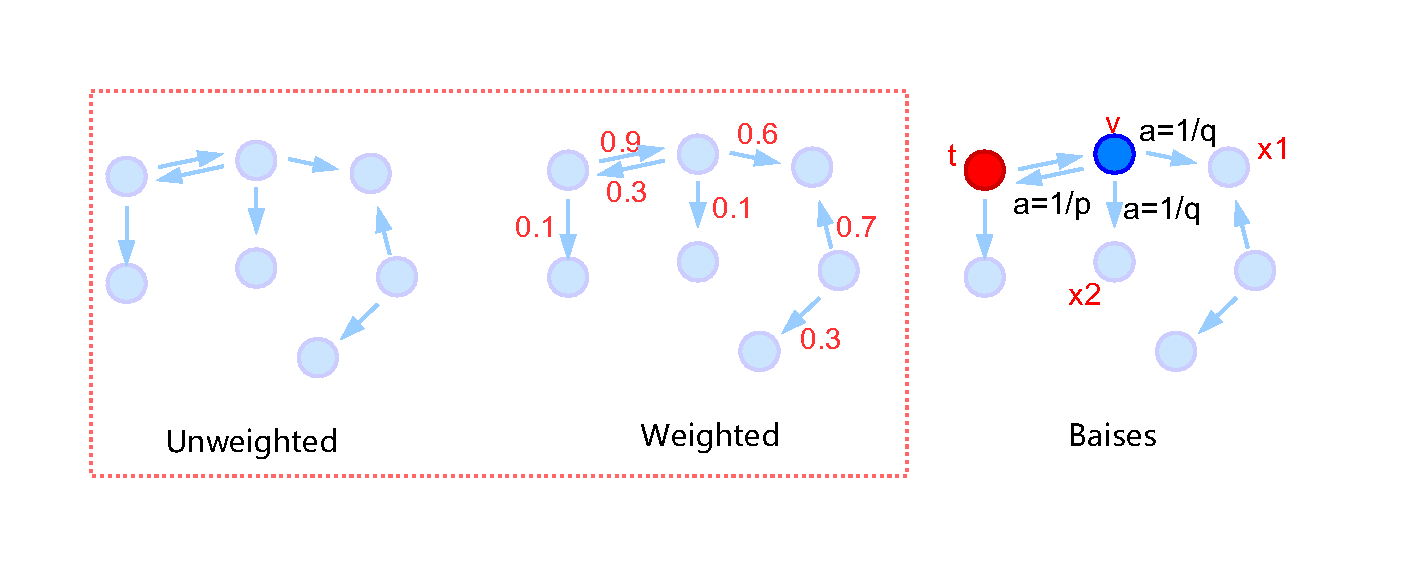
\includegraphics[width=0.5\textwidth]{pic/graph.pdf}\\
    \caption{Unweighted, Weighted topological structure and the random walk bias}
    \label{two_graph}
\end{figure}

\subsubsection{measurement}
We can get the embedding for an entity $e_i$, that consists of attributes information embedding($\overrightarrow {va}_i$) and
topological structure embedding($\overrightarrow {vt}_i$). Formally, we refer to the relatedness of entity-to-entity as:

\begin{small}
    \begin{equation}
        f_e(e_i, e_j) = \alpha cos({\overrightarrow {va}_i, \overrightarrow {va}_j}) 
        + (1-\alpha)cos(\overrightarrow {vt}_i,\overrightarrow {vt}_j)
    \end{equation}
\end{small}where $\alpha \in [0,1]$ is to adjust the weights of two parts.


\subsection{Word Semantic Relatedness \emph{F}}
We consider three layers for final semantic relatedness measurement including word-to-word, word-to-entity and entity-to-entity.
The word-to-entity and entity-to-entity are combined as concept-layer relatedness $F_c(w_i, w_j)$, and we refer to
word-to-word to word-layer relatedness named $F_w(w_i, w_j)$. Formally, We have:

\begin{small}
    \begin{equation}
        F_c(w_i, w_j) = \sum_{e_i \in E_i}^{ }\sum_{e_j \in E_j}^{ }f_{we}(w_i, e_i)f_e(e_i, e_j)f_{we}(w_j, e_j)
    \end{equation}
\end{small}in which $E_i$ is the entities set that is associated with word $w_i$.
The final word semantic relatedness measurement are:

\begin{small}
    \begin{equation}
        F(w_i, w_j) = \varphi F_w(w_i, w_j) + (1 - \varphi) F_c(w_i, w_j)
    \end{equation}
\end{small} $\varphi \in [0,1]$ trades off the weight of $F_w$ against $F_c$.





  \section{Experiment}
In this section, we conduct extensive experiments on different datasets which
contain the semantic measurement by human perceptions. We compute the Spearman
correlation coefficient between results of experiments and scores of human judgement
to evaluate the performance of our model. The model is implemented on 
cpu Core-7-7700K@4.20GHz$\times$8 machine with 16GB memory and ArchLinux platform.
 
\subsection{Dataset}
To evaluate models for semantic relatedness measurement, a common approach is to compare
the scores from the model and the scores provided by humans performing the same task.
This approach provides a model-independent way for evaluating measures of relatedness.
A good number of datasets record the scores of human quantitative judgement
for semantic relatedness such as \emph{MC-30}\cite{MC30/Miller02}, \emph{RG-65}\cite{RG65/RubensteinG65}, 
\emph{REL-122}\cite{acl/SzumlanskiGS13}, \emph{MEN}\cite{MEN/BruniTB14}, 
\emph{YP-130}\cite{YP130/Yang06verbsimilarity}, \emph{WS}\cite{ws/AgirreAHKPS09},
\emph{wordsim-353}\cite{wordsim353/FinkelsteinGMRSWR02}
and so on. Some of these datasets are established with the measurement of 
similarity called \emph{similarity dataset}. Some others are \emph{relatedness dataset}.
Note that all these datasets are English-language words.

1)\emph{similarity dataset}:
\emph{MC-30}, \emph{RG-65}, \emph{YP-130} and \emph{wordsim-353} are all established for computing similarity.
\emph{RG-65} is the classical similarity dataset which contains 65 pairs of words.
\emph{MC-30} contains 30 pairs of words and is the subset of \emph{RG-65}.
\emph{YP-130} is established for computing verb similarity which contains 130 pairs of verb.
\emph{wordsim353} contains two parts that are annotated by different groups of annotators.
The first set (set1) contains 153 word pairs along with their similarity scores assigned by 13 subjects. 
The second set (set2) contains 200 word pairs, with their similarity assessed by 16 subjects.
All these above are mere similarity datasets which just consider a particular case of relatedness.
There is another hybrid dataset \emph{WS} contains two sets of English words pairs along
with human-assigned similarity and relatedness judgements, called \emph{WS-sim} and \emph{WS-Rel} separately.
\emph{WS-sim} contains 203 pairs of words along with similarity judgement,
and \emph{WS-rel} contains 252 along with relatedness judgement.

2)\emph{relatedness dataset}:
Compared to the similarity datasets, there are a small number of relatedness datasets such as
\emph{WS-Rel}, \emph{MEN} and \emph{REL-122}. \emph{WS-Rel} contains 252 pairs of words with
human-assigned relatedness judgements. \emph{MEN} contains 3000 pairs of words which do not
instruct the subjects about the difference between similarity and relatedness. 
Due to the great number of human-assigned relatedness judgements, \emph{MEN} can
be used to train and test computer algorithms implementing semantic similarity or relatedness measures.
We would not consider this collection in our experiments because of the illegibility of semantic measurement.
Another dataset \emph{REL-122} is a new relatedness norm, and contains a set of human-assigned relatedness scores
for 122 pairs of nouns.

The difference between similarity dataset and relatedness dataset is how human assign the score for a
given pair of words. A common example is the pair of words \emph{"wheels-car"}. The \emph{wheels} is more related
with the \emph{car}, but they are dissimilar. The paper \cite{acl/SzumlanskiGS13} created two additional experimental 
conditions in which subjects evaluated the relatedness of noun pairs from the similarity dataset \emph{MC-30}. We select 
ten pairs of words shown in table \ref{mc}. 

\begin{table}[]
    \centering
    \caption{Relatedness vs MC-30 similarity}
    \label{mc}
    \renewcommand\arraystretch{1.2}
    \setlength{\tabcolsep}{2.5mm}{
        \begin{tabular}{|lllll|}
        \hline
        \textbf{\#}  & \multicolumn{2}{l}{\textbf{Noun Pairs}} & \textbf{Sim.} & \textbf{Rel.} \\ \hline
        \textbf{1.}  & car              & automobile          & 3.92          & 4.00         \\
        \textbf{2.}  & gem              & jewel               & 3.84          & 3.98         \\
        \textbf{3.}  & coast            & shore               & 3.70          & 3.97         \\
        \textbf{4.}  & journey          & car                 & 1.16          & 3.00         \\
        \textbf{5.}  & forest           & graveyard           & 0.84          & 2.01         \\
        \textbf{6.}  & coast            & hill                & 0.87          & 1.59         \\
        \textbf{7.}  & shore            & woodland            & 0.63          & 1.63         \\
        \textbf{8.}  & lad              & wizard              & 0.42          & 2.12         \\
        \textbf{9.}  & crane            & implement           & 1.68          & 0.90         \\
        \textbf{10.} & noon             & string              & 0.08          & 0.14         \\ \hline
        \end{tabular}
    }
\end{table}
We can see that the relatedness for pairs that are related but
dissimilar(e.g., \emph{journey-car} and \emph{forest-graveyard}). 
This indicates that asking subjects to evaluate “similarity” instead of “relatedness” can
significantly impact the results in studies of semantic relatedness measurement.
However, previous researchers do not consider the semantic difference among some datasets.
For example, in \cite{ijcai/GabrilovichM07}, \cite{textgraphs/YehRMAS09}, \cite{aaai/Pirro12}
and so on, the researchers all regard the dataset \emph{MC-30} as relatedness dataset to conduct experiments.
Following these reasearches, the similarity dataset \emph{MC-30} and \emph{RG-65} would be leveraged in our experiments 
besides the relatedness datasets \emph{rel-122} and \emph{WS-rel}. Moreover, we extract the relatedness
scores from paper \cite{acl/SzumlanskiGS13}. And some of these pairs are shown in table \ref{mc} for dataset \emph{MC-30}.

For a given pair of words, we firstly get two sets of corresponding entities in DBPedia. 
Then we adopt a method of embedding to train the subgraph which is extracted from DBPedia
based on queried entities. Finally,  we get multiple relatedness scores after
a full link between two sets of entities. In order to better fit the judgement of human, we utilize a
weighted strategy to combine multiple relatedness scores of pairwise entities.

\subsection{Parameter tuning}
We can recall from section \ref{sec:train} and \ref{sec:measure} that there are some parameters
which may have an impact on semantic relatedness measurement. The final relatedness
socre would be affected by the dimension of vector as well as the number of entities associated with given words.
Besides, we tune the $\alpha$ parameter for the \emph{weighted} strategy on \emph{WS-rel} dataset.
We pick \emph{WS-rel} since there are not many comparison systems in literature that
report results on this dataset. Another reason is that the quantity of \emph{WS-rel} is
greater than other datasets. It is comprehensive for our parameter tuning using dataset \emph{WS-rel}.
Finally, we find the optimal values for $\alpha$ to be 7.

% For the impact for final score which is affected by the number of entities queried by given words, we
% show the variation trend of \emph{Spearman} correlation coefficient following the increase of queried entities.

As you can see by the line chart \ref{dim}, we exhibit the impact of dimensions of learnt
vector for relatedness measurement with \emph{closest} and \emph{weighted} strategy. 
We conduct results based on datasets which consist of
\emph{MC-Rel-30}, \emph{MC-Sim-30}, \emph{RG-65}, \emph{rel-122}, and \emph{WS-rel}, and we get the 
average values of the results in five datasets shown in the sixth line chart finally. It is obvious
that the we get the optimal relatedness scores when the dimension of vector is assigned to \emph{100}.

\begin{figure}
    \centering
    \subfigure[The impact of Dimension of vector for relatedness measure]{
        \label{dim}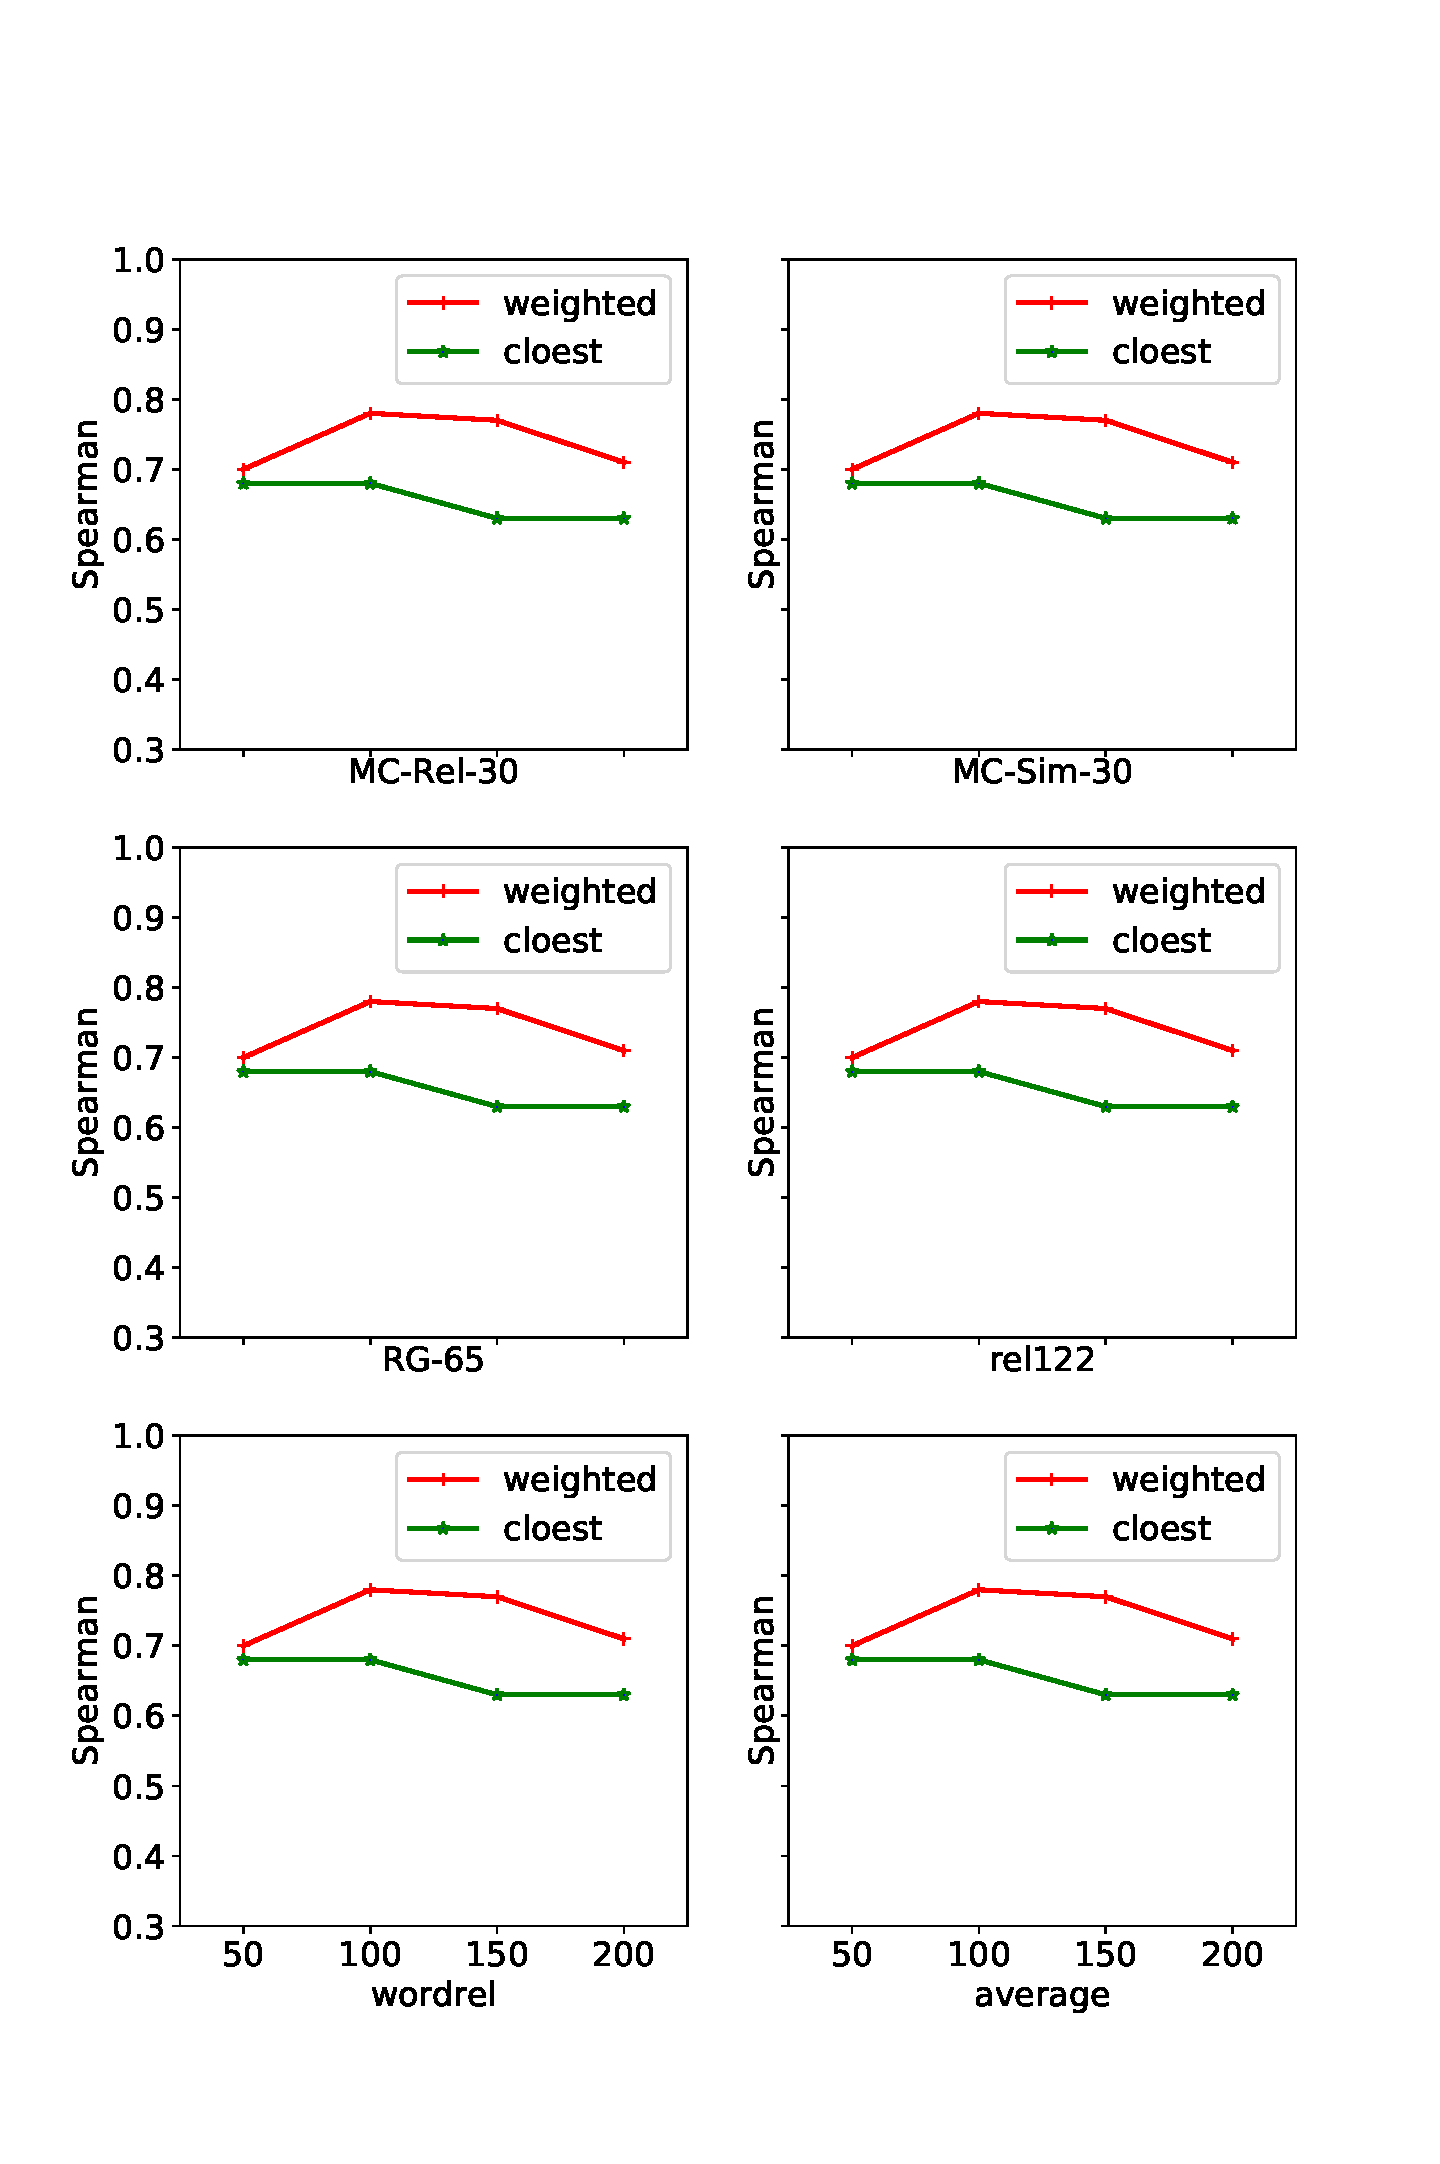
\includegraphics[width=55mm]{pic/dim.pdf}}
    \subfigure[The impact of the number of entities queried by given words]{
        \label{ent-num}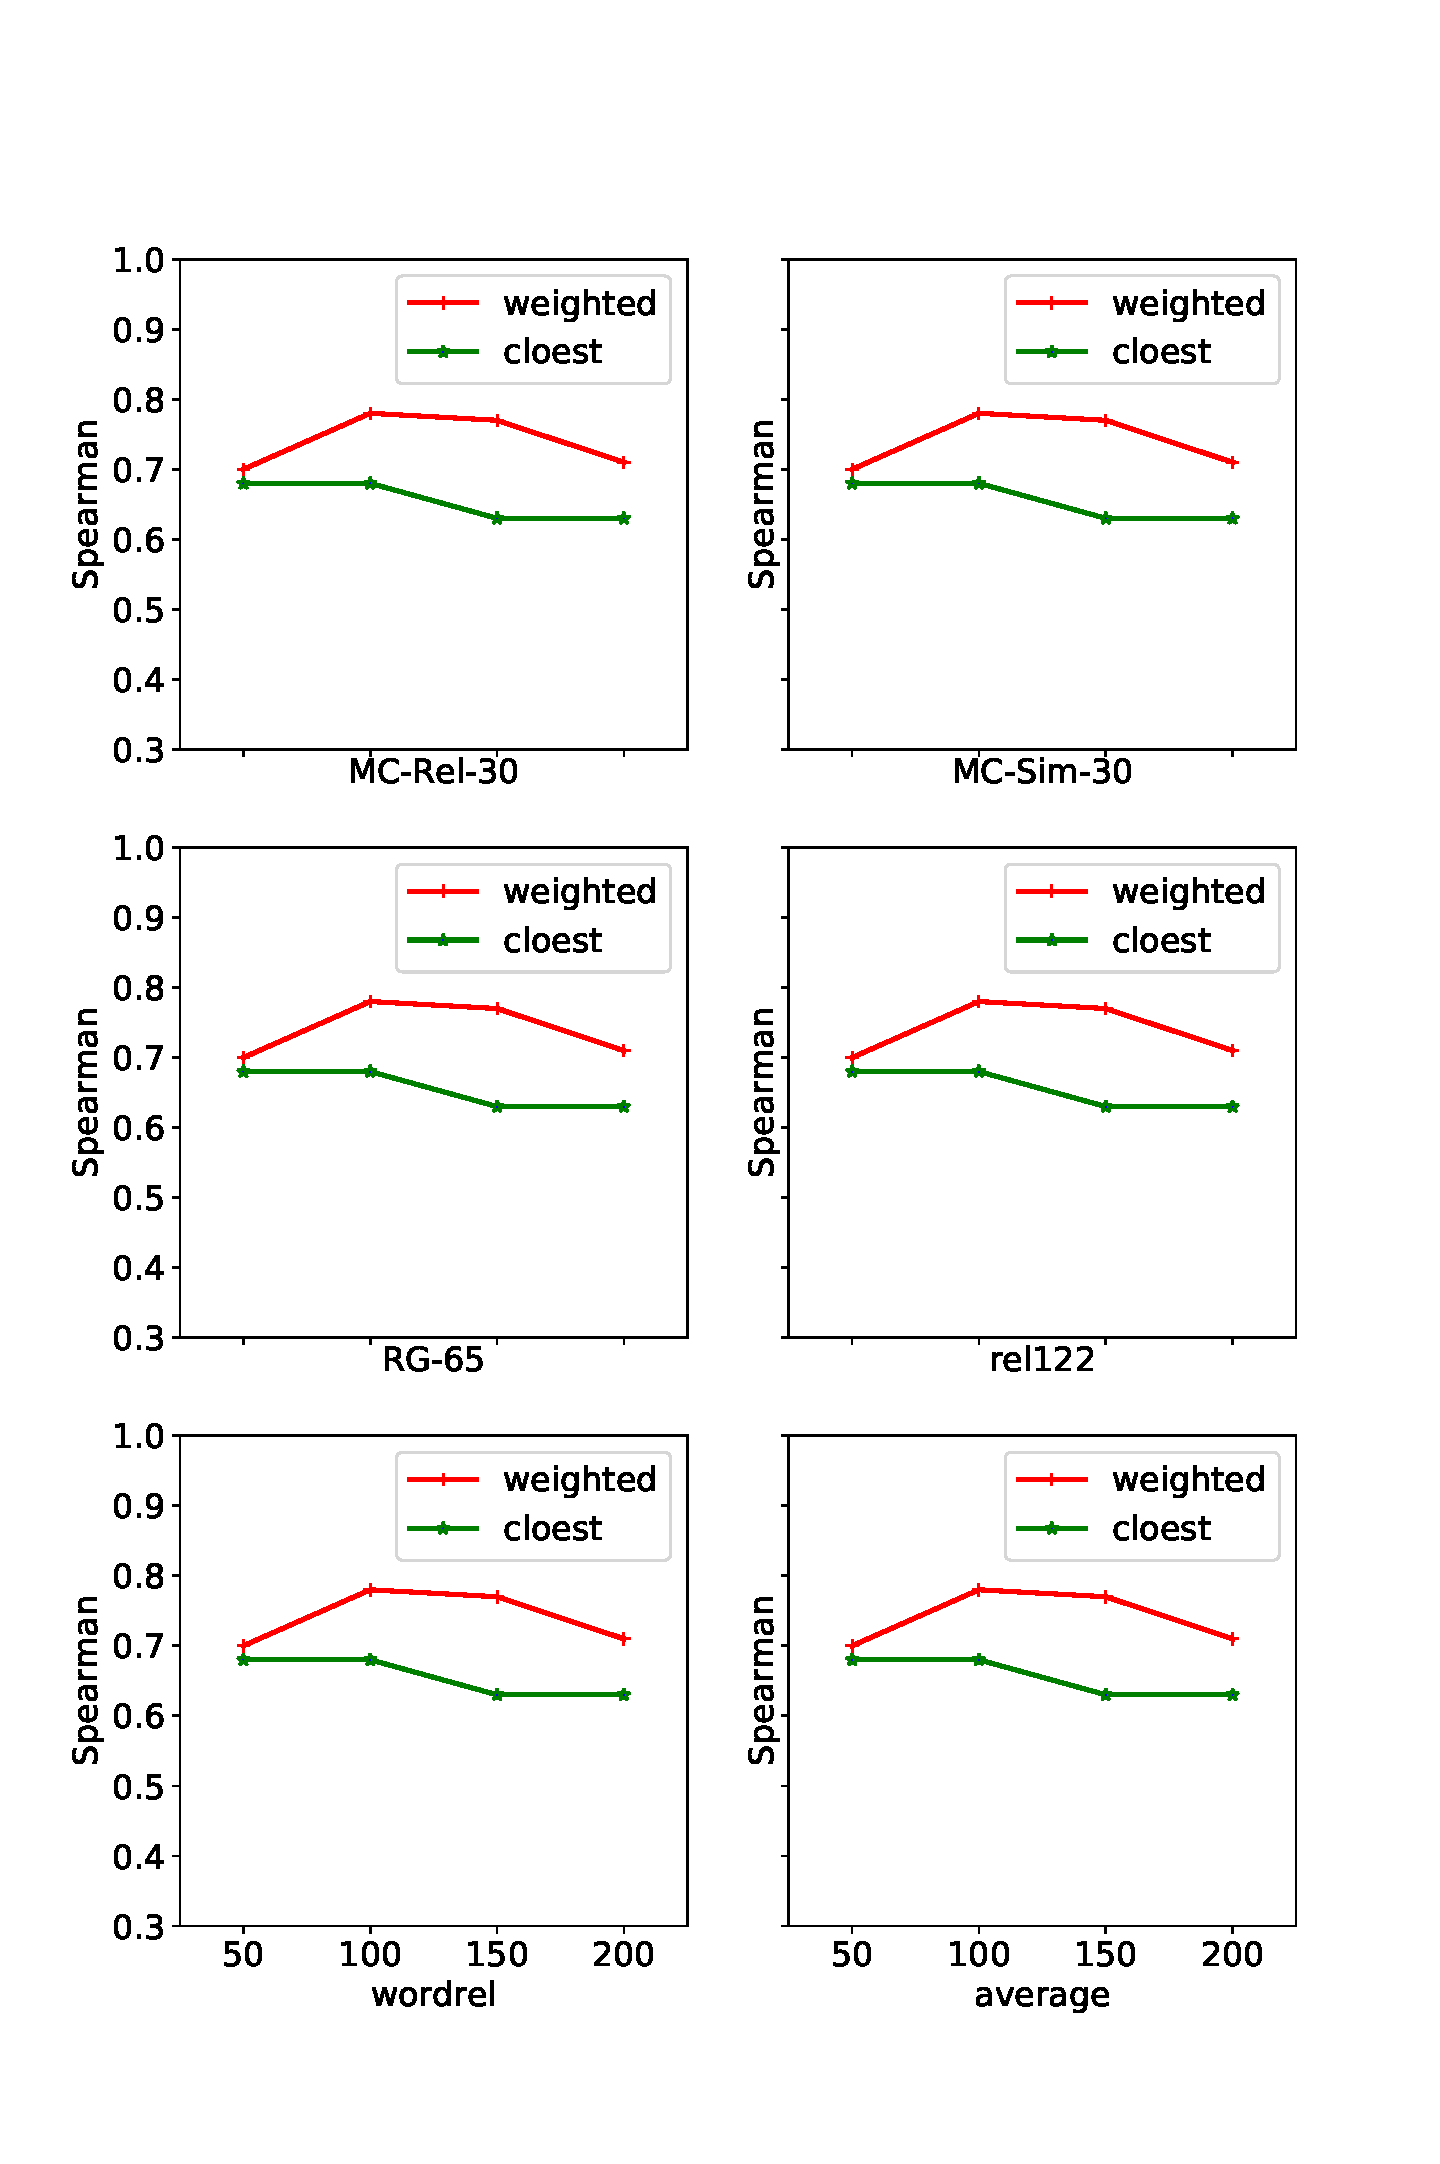
\includegraphics[width=55mm]{pic/dim.pdf}
    }
    \caption{Parameter Tuning}
\end{figure}


In the figure \ref{ent-num}, we draw the variation trend
of semantic relatedness scores following the increase of the quantity of entities queried by given words.
The slope of correlation coefficient curve rises gently with the increase of number of queried entities.
Distinguishingly, when the quantity of queried entities is greater than 5, the correlation coefficient
curve has a concave shown in pic \emph{X} because extra and overmuch entities would bring noise for the final
semantic relatedness scores.

\begin{table}[H]
    \centering
    \caption{Spearman correlation performance on five word similarity and relatedness datasets}
    \label{spearman}
    \renewcommand\arraystretch{1.15}
    \setlength{\tabcolsep}{2.5mm}{
        \begin{tabular}{lcllccl}
        \hline
        \multirow{2}{*}{\textbf{Measure}} & \multicolumn{5}{c}{\textbf{Dataset}}                                                                                          & \textbf{} \\ \cline{2-6}
                                        & \multicolumn{1}{l}{MC-rel-30} & MC-30 & RG-65                  & \multicolumn{1}{l}{rel122} & \multicolumn{1}{l}{wordrel} & Averrage  \\ \hline
        \textbf{WikiRelate!}              & --                            & 0.45          & 0.52                   & --                         & --                          &           \\
        \textbf{ESA}                      & --                            & 0.75          & 0.82                   & --                         & --                          &           \\
        \textbf{WLM}                      & --                            & 0.70          & 0.64                   & --                         & --                          &           \\
        \textbf{WikiWalk}                 & --                            & 0.61          & \multicolumn{1}{c}{--} & --                         & --                          &           \\
        \textbf{REWOrD}                   & --                            & 0.72          & 0.78                   & --                         & --                          &           \\ \hline
        \textbf{Pando-closest}            & \multicolumn{1}{l}{}          & 0.81          &                        & \multicolumn{1}{l}{}       & \multicolumn{1}{l}{}        &           \\
        \textbf{Pando-weighted}           & \multicolumn{1}{l}{}          & \textbf{0.85} &                        & \multicolumn{1}{l}{}       & \multicolumn{1}{l}{}        &           \\ \hline
        \end{tabular}
    }
\end{table}

Compared to previous method of semantic relatedness measurement, we run our model on five dataset
\emph{MC-Rel-30}, \emph{MC-Sim-30}, \emph{RG-65}, \emph{rel-122}, and \emph{WS-rel}, and report the
\emph{Spearman} correlation coefficient performance for the two strategies of our model. It can be
seen that our model proves to be highly reliable on semantic relatedness measurement tasks. Our model obtains
the best performance on most datasets. In addition, our approach in dataset \emph{MC-Rel-30} outperforms
the results in dataset \emph{MC-Sim-30} which proves that our model is more suitable for computing semantic
relatedness than similarity. 
  % \section{Related Work}
Computing semantic relatedness(SR) between two elements(words, sentences,
texts etc.) is a fundamental task for many applications in Natural Language
Processing(NLP) such as lexicon induction(\cite{aaai/QadirMGL15}), Named 
Entity Disambiguation{\cite{acl/HanZ10}}, Keyword Extraction
(\cite{ijcai/ZhangFW13}) and Information Retrieval(\cite{acl/GurevychMZ07}). 
Additionaly, computing semantic relatedness contributes other applications, 
for example, opinion spam problem (\cite{www/SandulescuE15}) and so on(+some example). 
In this paper we focus on computing semantic relatedness between two 
words in knowledge graph with neural network.


Semantic measures are mathematical tools used to estimate the strength of the 
semantic relationship between units of language, concepts or instances, through 
a (numerical) description obtained according to the comparison of information 
supporting their meaning. The semantic measures contain semantic relatedness,
semantic similarity, semantic distance. The semantic distance equal to semantic 
unsimilarity. The similarity is only one particular type of relatedness.
Comparison to similarity fails to give a complete view of a relatedness measures.


In this paper we computing semantic relatedness on the account of knowledge
graph. Computational of semantic relatedness is a superset of similarity.
The similarity is only one particular type of relatedness, comparison to
similarity fails to give a complete view of a relatedness measures.

Approaches to measuring semantic relatedness that use lexical
resources (instead of distributional similarity of words, 
e.g. Landauer and Dumais (1997) and Turney (2001)) transform
that resource into a network or graph and compute
relatedness using paths in it. Rada et al. (1989) traverse
MeSH, a term hierarchy for indexing articles in Medline,
and compute semantic relatedness straightforwardly in
terms of the number of edges between terms in the hierarchy.
Jarmasz and Szpakowicz (2003) use the same approach
with Roget’s Thesaurus while Hirst and St-Onge (1998) apply
a similar strategy to WordNet. Since the edge counting
approach relies on a uniform modeling of the hierarchy,
researchers started to develop measures for computing semantic
relatedness which abstract from this problem (Wu and
Palmer, 1994; Resnik, 1995; Leacock and Chodorow, 1998;
Finkelstein et al., 2002; Banerjee and Pedersen, 2003, inter
alia). Those researchers, however, focused on developing
appropriate measures while keeping WordNet as the de facto
primary knowledge source.

\cite{aaai/StrubeP06}
\cite{ijcai/GabrilovichM07}
\cite{www/RadinskyAGM11}

\cite{aaai/Pirro12}
\cite{aaai/NavigliP12}

\cite{acl/IacobacciPN15}

\cite{ijcai/SenJHMOMVWH15} domain specific semantic relatedness 


In this paper we focused on semantic relatedness, which
generalizes similarity by considering not only specialization
relations between words. The application of semantic
relatedness span different areas from natural language processing
(Patwardhan, Banerjee, and Pedersen 2003) to distributed
systems (Pirro, Ruffolo, and Talia 2008). In the Se- ´
8http://relwod.wordpress.com
9http://uniprot.bio2rdf.org/sparql
mantic Web context, some initiatives consider RDF predicates
for vocabulary suggestion (Oren, Gerke, and Decker
2007) while other (Freitas et al. 2011) exploit relatedness
for query answering over Linked Data. However, differently
from REWOrD none of them is specifically focused on computing
relatedness in the Web of Data.
Generally speaking, computational approaches to relatedness
exploit different sources of background knowledge
such as WordNet (e.g., (Resnik 1995; Budanitsky A 2001)),
MeSH (e.g., (Rada, Mili, and Bicknell 1989; Pirro and ´
Euzenat 2010)) or search engines (e.g., (Bollegala, Matsuo,
and Ishizuka 2007; Turney 2001)). Recently, Wikipedia
has been shown to be the most promising source of background
knowledge for relatedness estimation (Gabrilovich
and Markovitch 2007). Therefore we’ll consider approaches
exploiting Wikipedia as baseline for comparison.
WikiRelate! (Ponzetto and Strube 2007), given two words
first retrieves the corresponding Wikipedia articles whose titles
contain the words in input. Then, it estimates relatedness
according to different strategies among which comparing
the texts in the pages or computing the distance between
the Wikipedia categories to which the pages belong.
Explicit Semantic Analysis (Gabrilovich and Markovitch
2007) compute relatedness both between words and text
fragments. ESA derives an interpretation space for concepts
by preprocessing the content of Wikipedia to build
an inverted index that for each word, appearing in the corpus
of Wikipedia articles, contains a weighted list of articles
relevant to that word. Relevance is assessed by the
TFIDF weighting scheme while relatedness is computed by
the cosine of the vectors associated to the texts in input.
WLM (Milne and Witten 2008) instead of exploiting text
in Wikipedia articles, scrutinizes incoming/outgoing links
to/from articles. WikiWalk (Yeh et al. 2009) extends the
WLM by exploiting not only link that appear in an article
(i.e., a Wikipedia page) but all links, to perform a random
walk based on Personalized PageRank.
The most promising approach, in terms of correlation, is
ESA. However, ESA requires a huge preprocessing effort to
build the index, only leverages text in Wikipedia and does
not consider links among articles. Therefore, it may suffer
some problems when the amount of text available is not large
enough to build the interpretation vectors or when changing
the source of background knowledge.
  \section{Conclusion}
test.
  
  \bibliographystyle{aaai}
  \bibliography{aaai19}
  \end{document}